\documentclass[11pt,a4paper]{article}
\usepackage[utf8]{inputenc}
\usepackage[margin=1in]{geometry}
\usepackage{amsmath,amssymb}
\usepackage{booktabs}
\usepackage{graphicx}
\usepackage{xcolor}
\usepackage{listings}
\usepackage{hyperref}
\usepackage{microtype}
\usepackage{float}

\hypersetup{
    colorlinks=true,
    linkcolor=blue!70!black,
    citecolor=blue!70!black,
    urlcolor=blue!70!black
}

\lstset{
    basicstyle=\ttfamily\footnotesize,
    keywordstyle=\color{blue!80!black}\bfseries,
    stringstyle=\color{green!50!black},
    commentstyle=\color{gray},
    numbers=none,
    frame=single,
    rulecolor=\color{gray!40},
    breaklines=true,
    backgroundcolor=\color{gray!5},
    captionpos=b,
    tabsize=4
}

\title{\textbf{Mainrun Report}}
\author{Hugh Signoriello}
\date{}


\begin{document}
\maketitle


\section{Introduction}
This report details the architectural and optimisation improvements made to an autoregressive transformer model trained on Hacker News headline text to predict the next token. The Lllama-based transformer  acheives a minimum validation loss of around 1.223 on the hacker news dataset when trained on 7 epochs with a 10\% validation split.

\section{Changes Made}

To progress beyond the baseline GPT-style transformer architecture, I implemented a LLaMA-style transformer architecture broadly based on Meta's LLaMA model family. This architecture was chosen due to its demonstrated empirical performance advantages over standard GPT baselines across numerous language benchmarks \cite{llama}. It also offers improved training efficiency, delivering competitive performance with substantially fewer parameters compared to GPT-3 and PaLM architectures \cite{llama}. This parameter efficiency is especially advantageous given the operational constraint of a 7-epoch training limit and local compute availability. The overall LLaMA-style architecture defined in \texttt{llama\_model.py} has 22.97M parameters with 6 transformer layers, 8 attention heads, and an embedding dimension of $d_{\text{model}} = 512$. These parameters were found to be appropriate for the size of the Hacker News dataset, and small enough to allow for fast iteration but not large enough to cause overfitting. The overall architecture is outlined in Figure~\ref{fig:llama-3-architecture} below.

\begin{figure}[H]
\centering
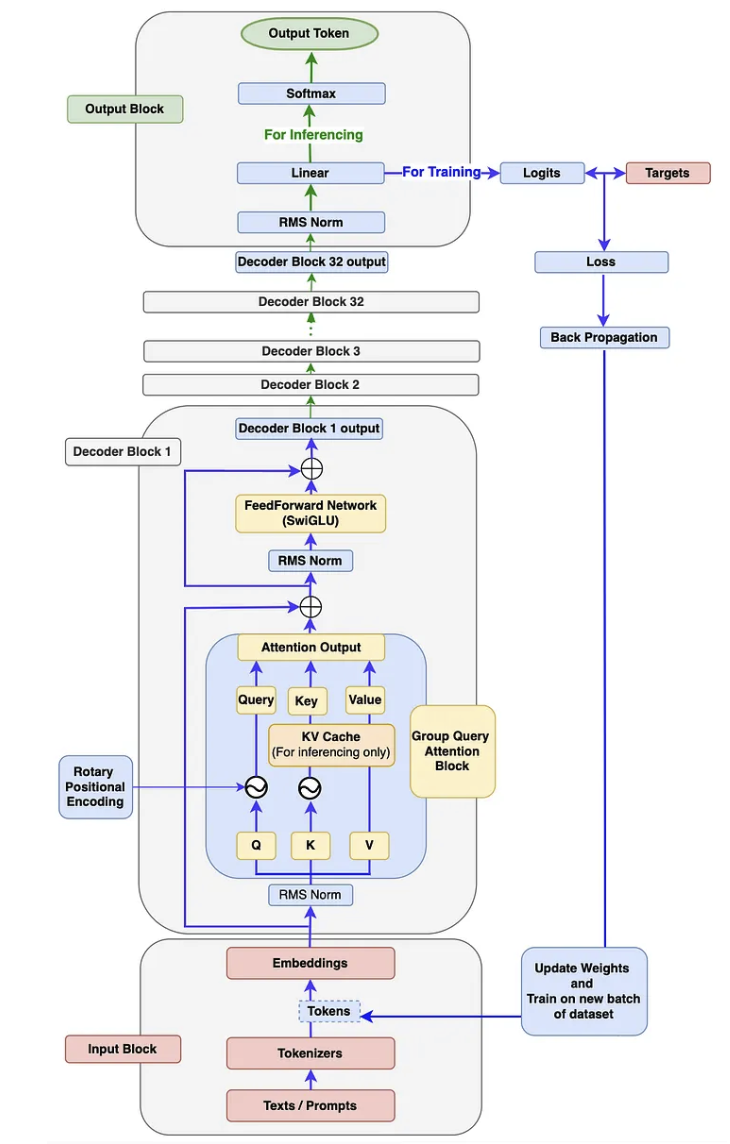
\includegraphics[width=0.6\textwidth]{docs/images/llama-3-architecture.png}
\caption{LLaMA-3 Architecture \cite{llama-3-guide}.}
\label{fig:llama-3-architecture}
\end{figure}

\subsection{Tokenisation}

The dataset loading,  Byte Pair Encoding (BPE) tokenizer training, and data batching logic remain the same as baseline and this logic was moved to \texttt{data.py} to seperate concerns. The BPE tokenization algorithm which is used in the official llama implementation \cite{llama} and is trained on 100,000 Hacker News titles and has a vocabulary size of 8000 tokens. Decreasing vocabulary from 16k to 8k tokens size led to reduced validation loss. Also infrequent words might be broken down into common subword tokens allowing the model to better generalise to unseen text and may give the model more capacity for tranfomer layers to learn dataset terminology with the reduced token vocabulary size.

\subsection{Root Mean Square Layer Normalisation (RMSNorm)}
I replaced standard LayerNorm with Root Mean Square Layer Normalisation (RMSNorm). Unlike standard LayerNorm, RMSNorm using pyTorch's \texttt{nn.RMSNorm} and is favoured as it is computationally simpler and only requires a single pass making it more efficient than LayerNorm \cite{rmsnorm}  which may imrprove training speed and stability of transformer training.


\subsection{SwiGLU Feed-Forward Network}
I replaced standard 2-layer GELU MLPs with Swish-Gated Linear Units (SwiGLU) \cite{swiglu}, as integrated into the \texttt{LlamaMLP} block. The SwiGLU activation function behaves similarly to ReLU on positive inputs, but outputs small negative values for negative inputs \cite{llama-3-guide} and Swish has been shown to outperform ReLU in many applications and it provides a smoother transition around 0, which may lead to faster training convergence. This is particulary advantageous considering the 7 epoch constraint. 

\begin{equation}
\text{SwiGLU}(x) = \left(\text{SiLU}(x W_{\text{gate}}) \odot (x W_{\text{up}})\right) W_{\text{down}}
\end{equation}


To maintain the parameter budget relative to standard $4 \times d_{\text{model}}$ MLPs, the intermediate hidden dimension was scaled by $\frac{2}{3} \times 4 d_{\text{model}} = \frac{8}{3} d_{\text{model}}$ following LLaMA specifications \cite{llama}:


\subsection{Rotary Position Embeddings (RoPE)}

The absolute positional embeddings were removed and replaced with rotary positional embeddings (RoPE) \cite{llama}. RoPE is a type of position encoding that maintains the order of tokens in sequences by incorporating both absolute position and relative position information among tokens \cite{llama-3-guide}. It performs positional encoding by rotating query and key representations using a rotation matrix. RoPE is advantageous because it naturally incorporates relative position dependency into the self-attention formulation, providing flexibility across sequence lengths and decaying inter-token dependency with increasing relative distance \cite{rope} compared to learned absolute embeddings. As a result of helping the transfomer genralise better to longer sequences and learn positional context more effectively than traditional absolute position enbeddings, RoPE embeddigns may decrease the loss function. The implementation was adapted from: \href{https://github.com/huggingface/transformers/blob/main/src/transformers/models/llama/modeling_llama.py}{Hugging Face Transformers \texttt{modeling\_llama.py}}. In thisn the code you are using (the rotate_half method), the vector is split down the middle. In this implementation the vector is split down the middle. The first half represents all the x-coordinates, and the second half represents all the y-coordinates for which the rotation matrix is applied. 

\section{Training Process and Hyperparameter Selection}

In the first few training runs I experimented with the training hyperpamaters to see how they affected validation loss, particularly on the GPT-style transformer architecture and then later experimented with these hyperparamaters on the Llama-based transformer training.

\begin{itemize}
    \item \textbf{Total steps:} The transformer trains on 100,000 Hacker News titles over 7 epochs, which equals  2,247 total steps.
    \item \textbf{Dropout:}  In earlier runs, specifically exp-05-llama I observed that validation loss began to increase around Epoch 5  with a minimum validation loss of 1.240 followed by increased validation loss while training loss continued to decrease, suggesting mild overfitting. To mitigate this and smooth the validation curve, a dropout rate of $0.05$ was introduced so that the network will randomly deactivate 5\% of its neurons  in a given layer during each training iteration, allowing the model to better learn generalised patterns and mitigate overfitting.
        
\item \textbf{Optimiser:} The suggested optimiser for the transfomer is AdamW \cite{attention-is-all-you-need}.  The hyperparameters for AdamW  with $\beta_1 = 0.9$, $\beta_2 = 0.95$, and $\epsilon = 10^{-8}$ are selected following LLaMA's suggested training specifications \cite{llama}. A weight decay of $\lambda = 0.1$ is applied selectively to all 2D weight matrices \cite{llama}. Since LLaMA does not have bias terms in its linear layers, all 1D parameters correspond to RMSNorm scale vectors; these are explicitly excluded from weight decay ($\lambda = 0.0$) and are reflected in the \texttt{optim\_groups} dictionary in \texttt{train.py}.
    
    \item \textbf{Scheduler:} While the original LLaMA models employ 2,000 warmup steps, this smaller-scale model is trained over fewer total steps. The warmup period was therefore scaled down proportionally to 200 steps or around 1\% of the total training steps. Having a warmup prevents early training instability and divergence when training deep transformers with adaptive gradient optimisers like AdamW. 
    
    Following warmup, a cosine annealing schedule decays the learning rate down to 10\% of its peak value ($\eta_{\text{min}} = 0.1 \times \text{lr}$) \cite{llama}.
The cosine decay helps smoothly curve the learning rate downwards following a cosine function until the end of training, this helps prevent the model from exiting a good local minimum when the learning rate is at its maximum.
          


% Also as llama does not use bias, 
    
    \item \textbf{Hardware:} I trained the transformer on Apple Silicon MPS on my M4 mac reduce runtime leading to a significant speedup around five-fold over CPU execution when running in Docker container.

\end{itemize}

\section{Experimental Results}
Table~\ref{tab:results} summarises training iterations for various experiments and training logs for experiments can be found in \texttt{mainrun/logs} which list the hyperparameters and training metrics. I documented the various experiments and hyperparamater changes for each experiment in \texttt{docs/Training Log.md} as I found ways to iteratively improve the model's validation loss.

\begin{table}[htbp]
\centering
\resizebox{\textwidth}{!}{%
\begin{tabular}{@{}llcccc@{}}
\toprule
\textbf{Exp ID} & \textbf{Architecture \& Setup} & \textbf{LR} & \textbf{Params} & \textbf{Train Loss} & \textbf{Val Loss} \\
\midrule
Baseline & GPT-2, SGD, vocab-size 16k, block 128 & $6.0 \times 10^{-3}$ & $ 27.2$M & 8.179 & 1.754 \\
exp-001-hp & GPT-2, SGD, vocab-size 8k, block 64 & $1.0 \times 10^{-3}$ & $ 23.0$M & 8.223 & 2.025 \\
exp-002-hp & GPT-2, AdamW, vocab-size 16k, block 128, 0.1 dropout  & $6.0 \times 10^{-4}$ & $ 27.2$M & 5.802 & 1.291 \\
exp-003-hp & GPT-2, AdamW, vocab-size 8k, block 32 & $8.0 \times 10^{-4}$ & $ 23.0$M & 4.480 & 1.270 \\
exp-004-llama & LLaMA & $8.0 \times 10^{-4}$ & $22.97$M & 4.110 & 1.243 \\
exp-005-llama & LLaMA, Warmup + DecayWarmup & $6.0 \times 10^{-4}$ & $22.97$M & 3.656 & 1.252 \\
\textbf{exp-006-llama} & \textbf{LLaMA, Warmup + Decay, Dropout 0.05} & $\mathbf{6.0 \times 10^{-4}}$ & $\mathbf{22.97}$\textbf{M} & \textbf{4.035} & \textbf{1.223} \\
\bottomrule
\end{tabular}%
}
\caption{Validation loss progression across training runs within the 7-epoch limit.}
\label{tab:results}
\end{table}

\clearpage
\begin{thebibliography}{9}
\bibitem{llama} Touvron, H., et al. (2023). \textit{LLaMA: Open and Efficient Foundation Language Models}. arXiv:2302.13971.
\bibitem{attention-is-all-you-need} Vaswani, A., et al. (2017). \textit{Attention Is All You Need}. NeurIPS.
\bibitem{rope} Su, J., et al. (2021). \textit{RoFormer: Enhanced Transformer with Rotary Position Embedding}. arXiv:2104.09864.
\bibitem{swiglu} Shazeer, N. (2020). \textit{GLU Variants Improve Transformer}. arXiv preprint arXiv:2002.05202.
\bibitem{rmsnorm} Zhang, B., \& Sennrich, R. (2019). \textit{Root Mean Square Layer Normalization}. NeurIPS.
\bibitem{llama-3-guide} Tamang, M. (2024). \textit{Build Your Own LLaMA 3 Architecture from Scratch Using PyTorch}. Towards AI. \url{https://pub.towardsai.net/build-your-own-llama-3-architecture-from-scratch-using-pytorch-2ce1ecaa901c}
\end{thebibliography}

\end{document}
